
\section{Simulation}\label{sec:simulation}
This section examples four main challenges for pose and torque control of an object, arranged in increasing difficulty.  Each task uses a PD controller that uses the swarm's mean position and mean velocity to regulate the swarm's mean position,  as in \cite{ShahrokhiIROS2015}. The control input is the global force applied to each robot:
\begin{align}
u_x &= K_{p}(goal_x - \bar{x}) + K_{d}(0-\bar{v}_x) \nonumber\\
u_y &= K_{p}(goal_y  - \bar{y}) + K_{d}(0-\bar{v}_y)  \label{eq:PDcontrolPosition}
\end{align}
here $K_{p}$ is the proportional gain, and $K_{d}$ is the derivative gain.  
The swarm's average position is $[\bar{x},\bar{y}]^T$ and mean velocity is $[\bar{v}_x,\bar{v}_y]^T$.  
Each task uses a different algorithm to select the swarm's goal position $[goal_x,goal_y]^T$.

\paragraph{Pure torque control} \label{sec:simulationPureTorque}
An object with a pivot point can rotate, but not translate. A door is a common example of an object with a pivot. A door can have an angular velocity but cannot translate. 
 If there was only one robot touching the object, the robot should push at the point which maximizes the moment arm, at the extreme end of the object furthest from the pivot point.
The optimal pushing location provides the maximum force, because it maximizes  $r$ in \eqref{eq:torque}.
However, given a swarm of robots, maximizing $r$ is no longer the optimal solution.  
If the swarm hits the object with its mean position at the extreme edge, half of the robots will miss the object and  the swarm will be torn apart.
Because few robots remain,  the force is significantly decreased and torque is not maximized.
 In our simulation, the swarm applies torque until the swarm's mean position is beyond the object.  At this point, the swarm will be regathered in a corner before returning to torque control, a time-consuming task. 
 The key parameter of interest for a hinged door of length $L$ is $C$, the position along the door where the mean of the swarm will push.  The swarm is directed toward 
 
\begin{align}\nonumber
goal_x &= O_x + C \sin(O_{\theta}) \\
goal_y &= O_y + C \cos(O_{\theta})  \label{eq:TorqueControl}
\end{align}

 Fig. \ref{fig:LFig} illustrates how different values of $C$ result in different rates of turning. These simulations tested $C = \{1/2, 3/4, 5/8, 1\}L$  The fastest turning rates occurred with  $C =  5/8L$. Code is available at \cite{Shahrokhi16torque}.



\begin{figure}
\begin{center}
	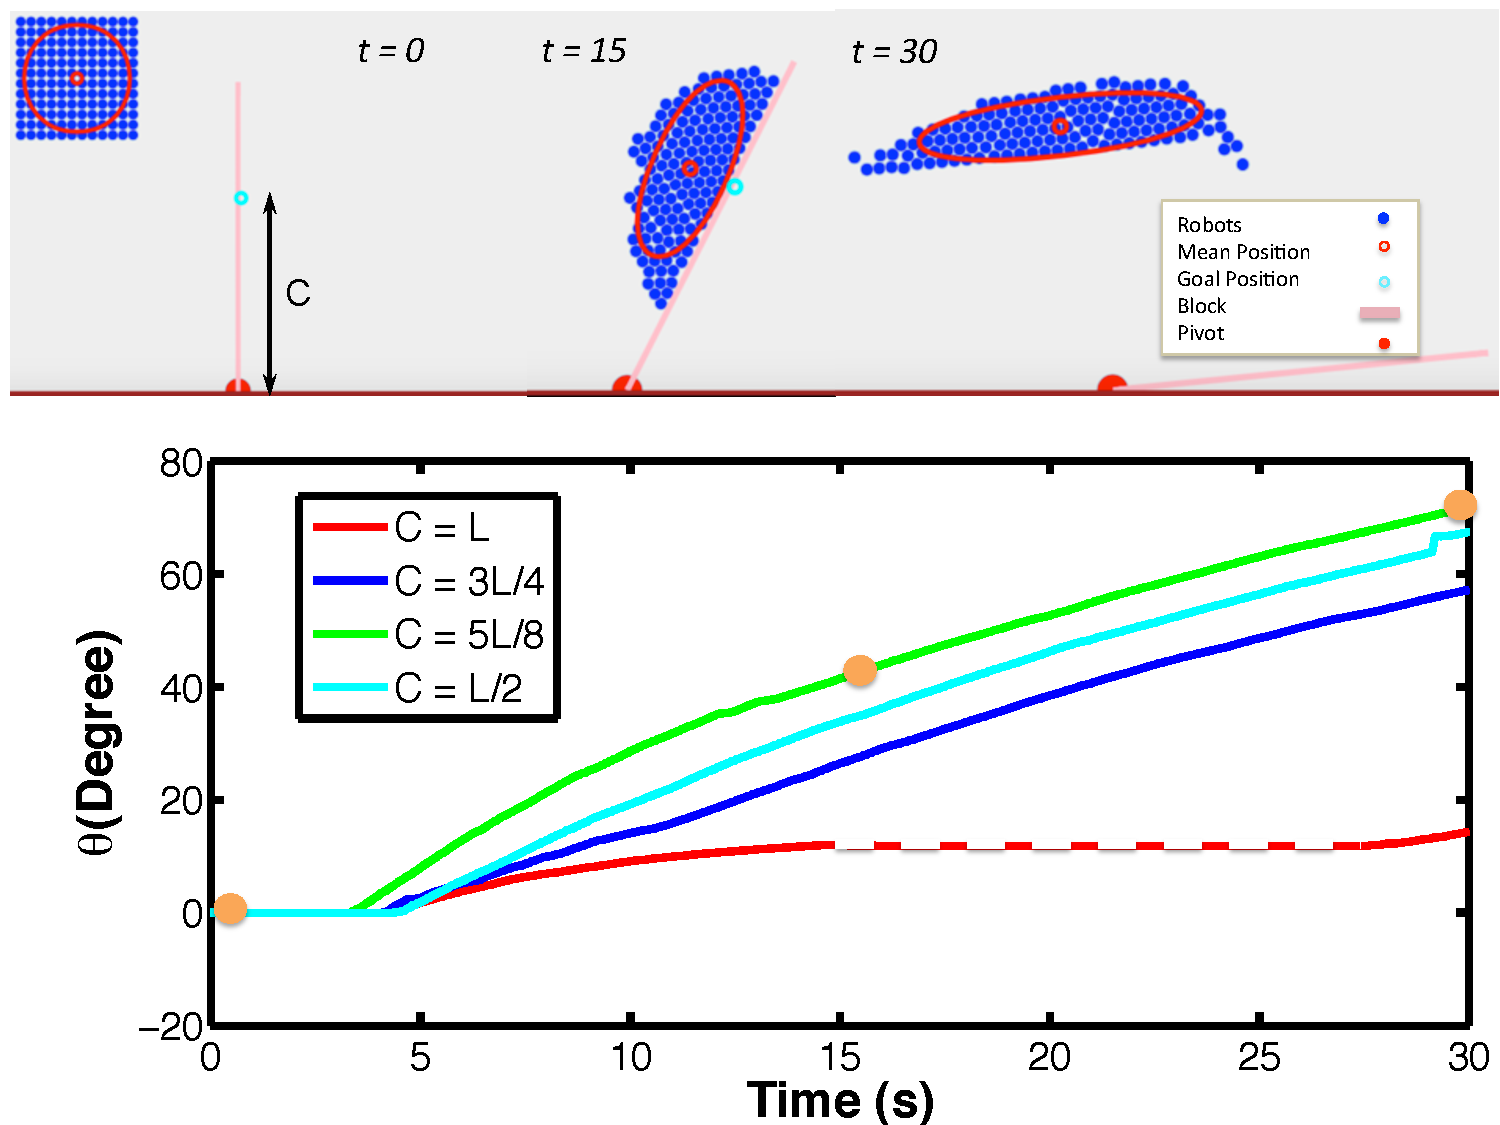
\includegraphics[width=\columnwidth]{LFig.pdf}
\end{center}
\vspace{-1em}
\caption{\label{fig:LFig}
Simulation results from a swarm applying force to a hinged door. 
The swarm mean is steered toward a point $C$ units along the object from the pivot point. The red dashed line indicates the times that the swarm was in variance control mode.
 Simulation used 144 robots of diameter $0.2$ m with a standard deviation of less than $1.5$ m and an object length of $6$ m.
}
\vspace{-1em}
\end{figure}


\paragraph{Orientation of the object}
These simulations used a uniform density rectangle as the object. This object was 30$\times$ larger than the robots.
Using the pure torque control discussed in the previous paragraph, the orientation of the object can be controlled by applying force. 
The rectangular object is not pivoted, so it moves in addition to rotating. 
 The swarm still may split into multiple components.
  We use the hysteresis variance control from \cite{ShahrokhiIROS2015}  to gather the swarm when its variance grows too large. 
  The following control law chooses a goal position to regulate the orientation of the object.  In the following equation, $O_{\theta}$ is the orientation of the object's major axis. The object COM is at $(O_x,O_y)$.

Let $O_{\theta}$ = the orientation of the object's major axis, measured from the world $x$-axis.
\begin{align}\nonumber
goal_x = O_x +  K_{orient}  (O_{\theta} - goal_\theta ) \cos(O_{\theta}) \\
goal_y = O_y +  K_{orient}  ( O_{\theta} -goal_\theta  ) \sin(O_{\theta})
\end{align}
Here $K_{orient}$ is a positive gain on the control input.  


\begin{figure}
\begin{center}
	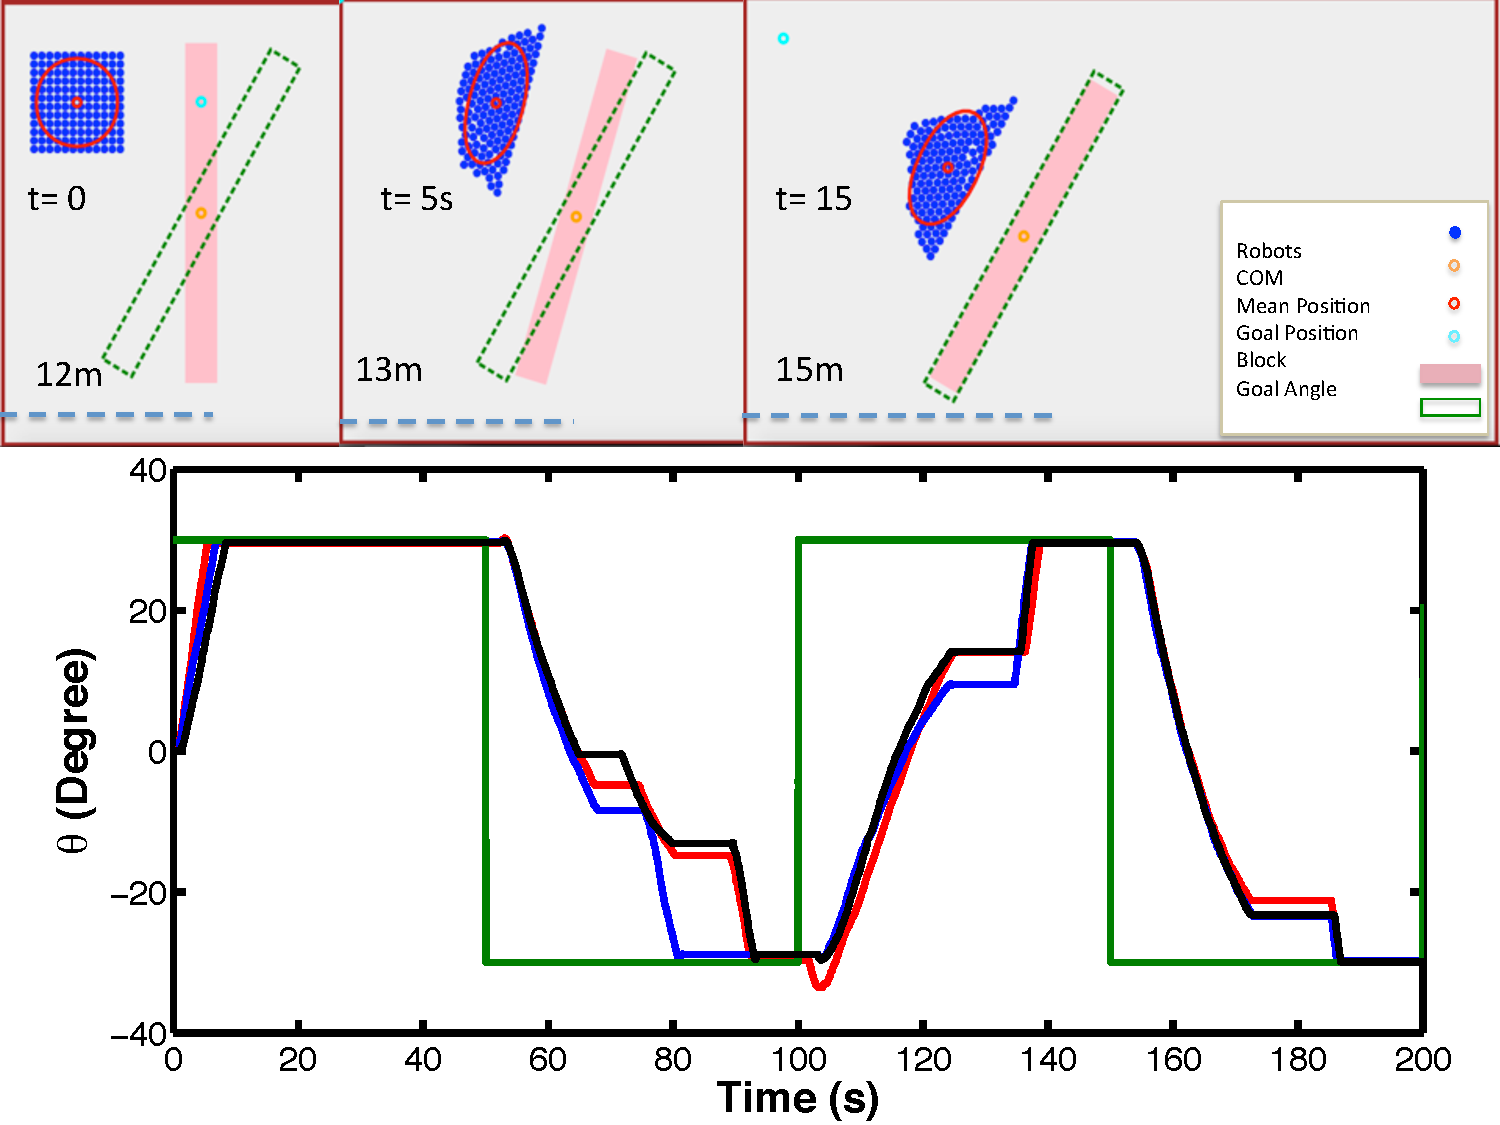
\includegraphics[width=\columnwidth]{Orientation.pdf}
\end{center}
\vspace{-1em}
\caption{\label{fig:OrientCont}
Plot demonstrating  orientation control of a rectangular object. The green line is the goal orientation.   When the plot traces are constant the swarm is no longer pushing the object and instead is being regathered in a corner of the workspace until the variance is below a desired threshold. 
}
\vspace{-1em}
\end{figure}

Fig. \ref{fig:OrientCont} illustrates this controller with different starting positions. When the plot traces are constant the swarm is no longer pushing the object and instead is being regathered in a corner of the workspace. Code is available at \cite{Shahrokhi16Orient}.

\paragraph{Straight translation while regulating object orientation} \label{para:PureTranslation}

When the total force is applied perpendicular to the object and in line with the center of mass, according to Eq. \eqref{eq:torque} there will be no torque. 
The following goal position for the mean position of the swarm regulates the object's orientation using $\Delta \theta$ for proportional feedback  to determine where to apply force.
$\Delta_\theta = goal_\theta - O_\theta$ is the difference between the goal angle and the current object angle.
 $K_\tau$ is a constant and $(O_x,O_y)$ is the position of the object's COM.
\begin{align}
goal_x &= O_x \nonumber \\
goal_y &= K_\tau \Delta\theta + O_y  \label{eq:TranslationAndOrientation}
\end{align}

 Fig. \ref{fig:Straight} shows how $\Delta \theta$ converges to zero with different initial configurations of the swarm. When the swam is above or below of the object the swarm applies a torque to the object. Code is available at \cite{Shahrokhi16translation}.
 
 
\begin{figure}
\begin{center}
	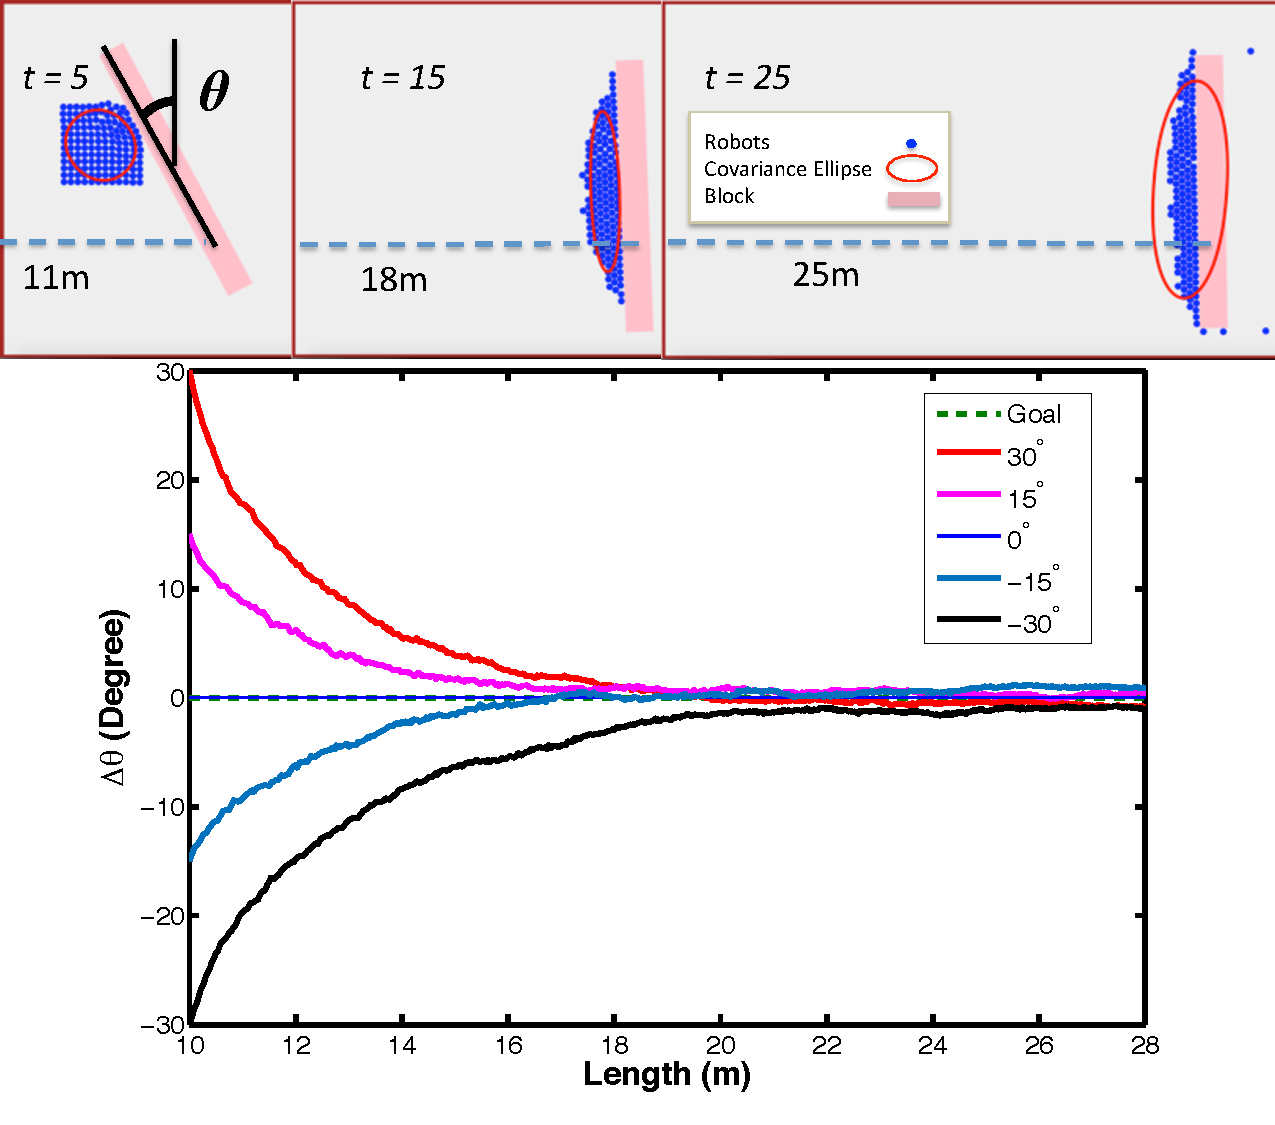
\includegraphics[width=\columnwidth]{Straight.pdf}
\end{center}
\vspace{-1em}
\caption{\label{fig:Straight}
In this task, the swarm pushed the object in the $+x$ direction while trying to regulate the orientation to $goal\theta = 0^\circ$.
 The swarm can push the object without changing its orientation only if it pushes along a line intersecting the COM of the object.  A feedback control law regulates the object's orientation.
}
\vspace{-1em}
\end{figure}

\paragraph{Line following with perpendicular orientation} \label{para:PureTranslation}
This task designs a control law that, given an arbitrary line, will push an object's COM onto that line and regulate the object's orientation to be perpendicular to that line.
Any line can be parameterized in the form $ax+by+c =0$,  which gives the locus of $(x,y)$ points along the line.  The point on this line nearest to the swarm COM $(O_x,O_y)$ is $P$:

%Assume an arbitrary line that if the object face that direction, the swarm should apply perpendicular force to the object to get to the desired location with the desired orientation.  We want to keep the object on the trajectory while the orientation of the object is also kept as desired. For this purpose, we have to find the intersection of the object orientation axis and the line. If the equation of the line is $ax+by+c =0$, and we name this point $P$, it can be found as:

\begin{align}
P_x &= \frac{b(bO_x-aO_y)-ac}{a^2 + b^2},\\ \nonumber
P_y &= \frac{a(-bO_x+aO_y)-bc}{a^2 + b^2}
\end{align}

%Then for keeping the object on trajectory, we will have the following goal position for correcting both perpendicular error and angle error while pushing the object:

The following control law regulates the goal position for the swarm COM to push the object COM onto the line and regulates the object angle.

\begin{align}
goal_x &= O_x+ K_p (O_x-P_x)+ K_\tau \frac{O_x-P_x}{||O_x-P_x||}\Delta\theta \nonumber \\
goal_y &= O_y+ K_p (O_y-P_y)+ K_\tau \frac{O_y-P_y}{||O_y-P_y||}\Delta\theta \label{eq:Regulate}
\end{align}

Fig. \ref{fig:Linear} shows the position and orientation over time 
while line following with perpendicular orientation.
The goal position for the swarm is based on the nearest point to COM in the line.
 When the swarm is in variance control mode, the goal position and COM position does not change. Fig. \ref{fig:LinearScreenShots} contains screenshots of this simulation. Code is available at \cite{Shahrokhi16TorqueLine}.

\begin{figure}
\begin{center}
	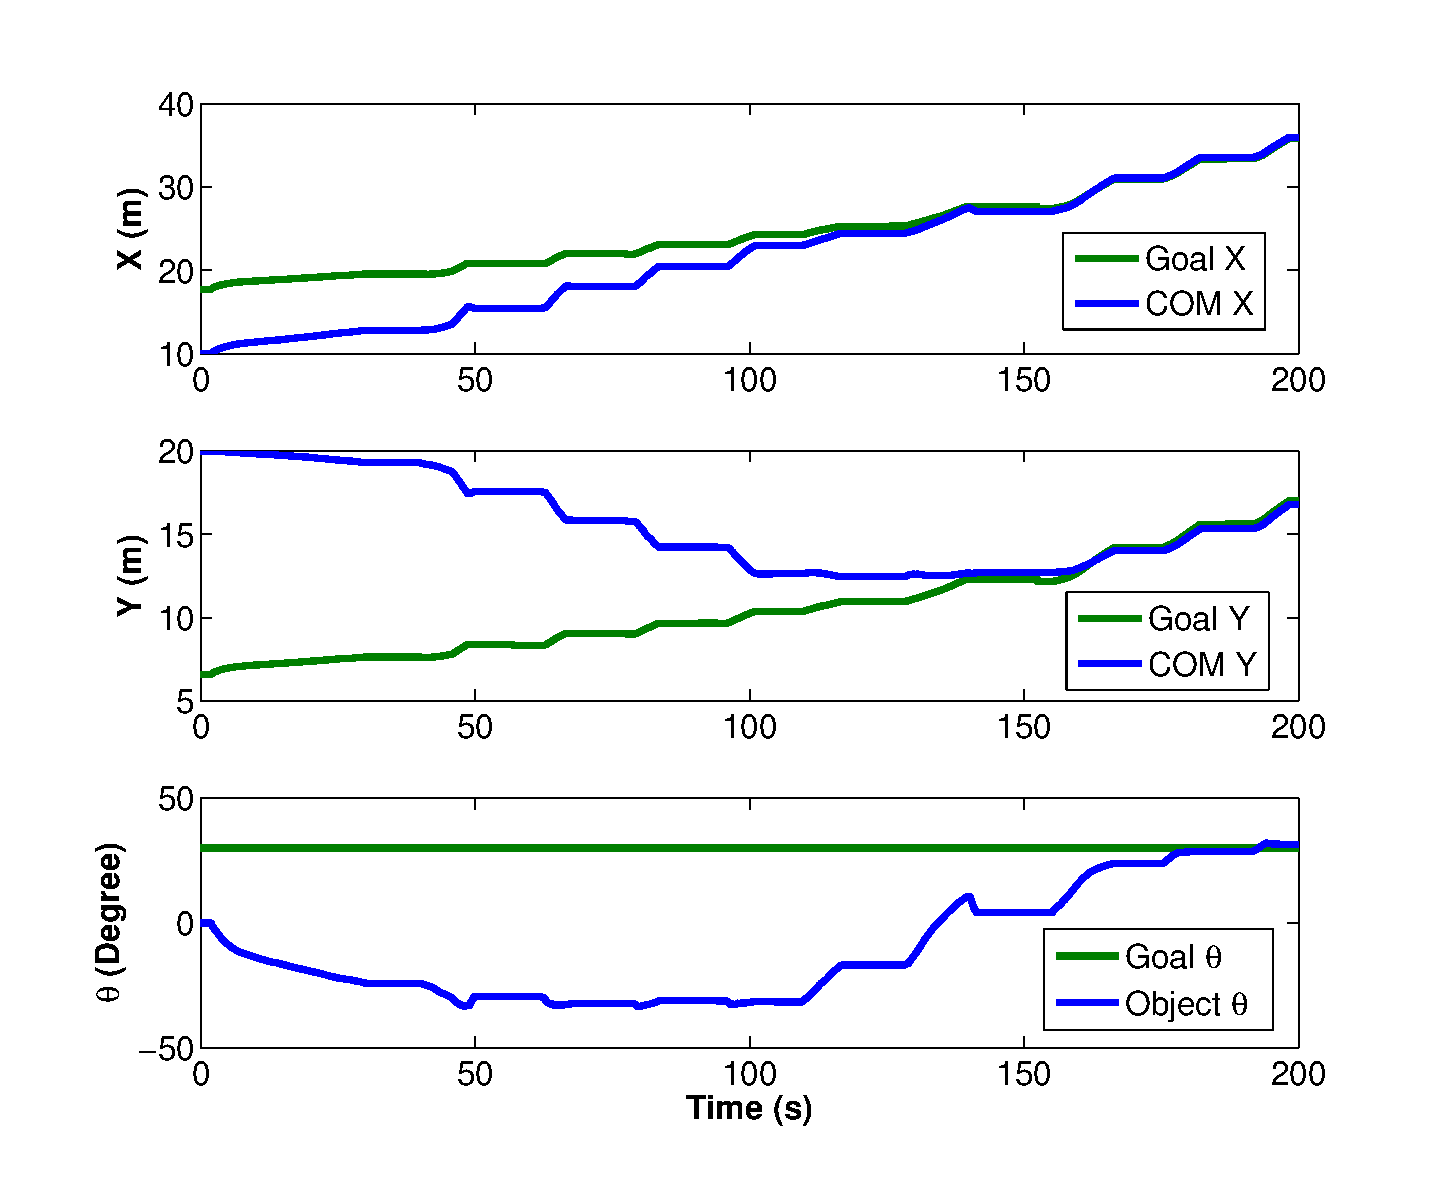
\includegraphics[width=1.07\columnwidth]{Linear.eps}
\end{center}
\vspace{-2em}
\caption{\label{fig:Linear} 
Following an arbitrary line with perpendicular orientation. This control law would keep the object on the line, while it regulates its orientation.
}
\vspace{-1em}
\end{figure}

\begin{figure*}
\centering

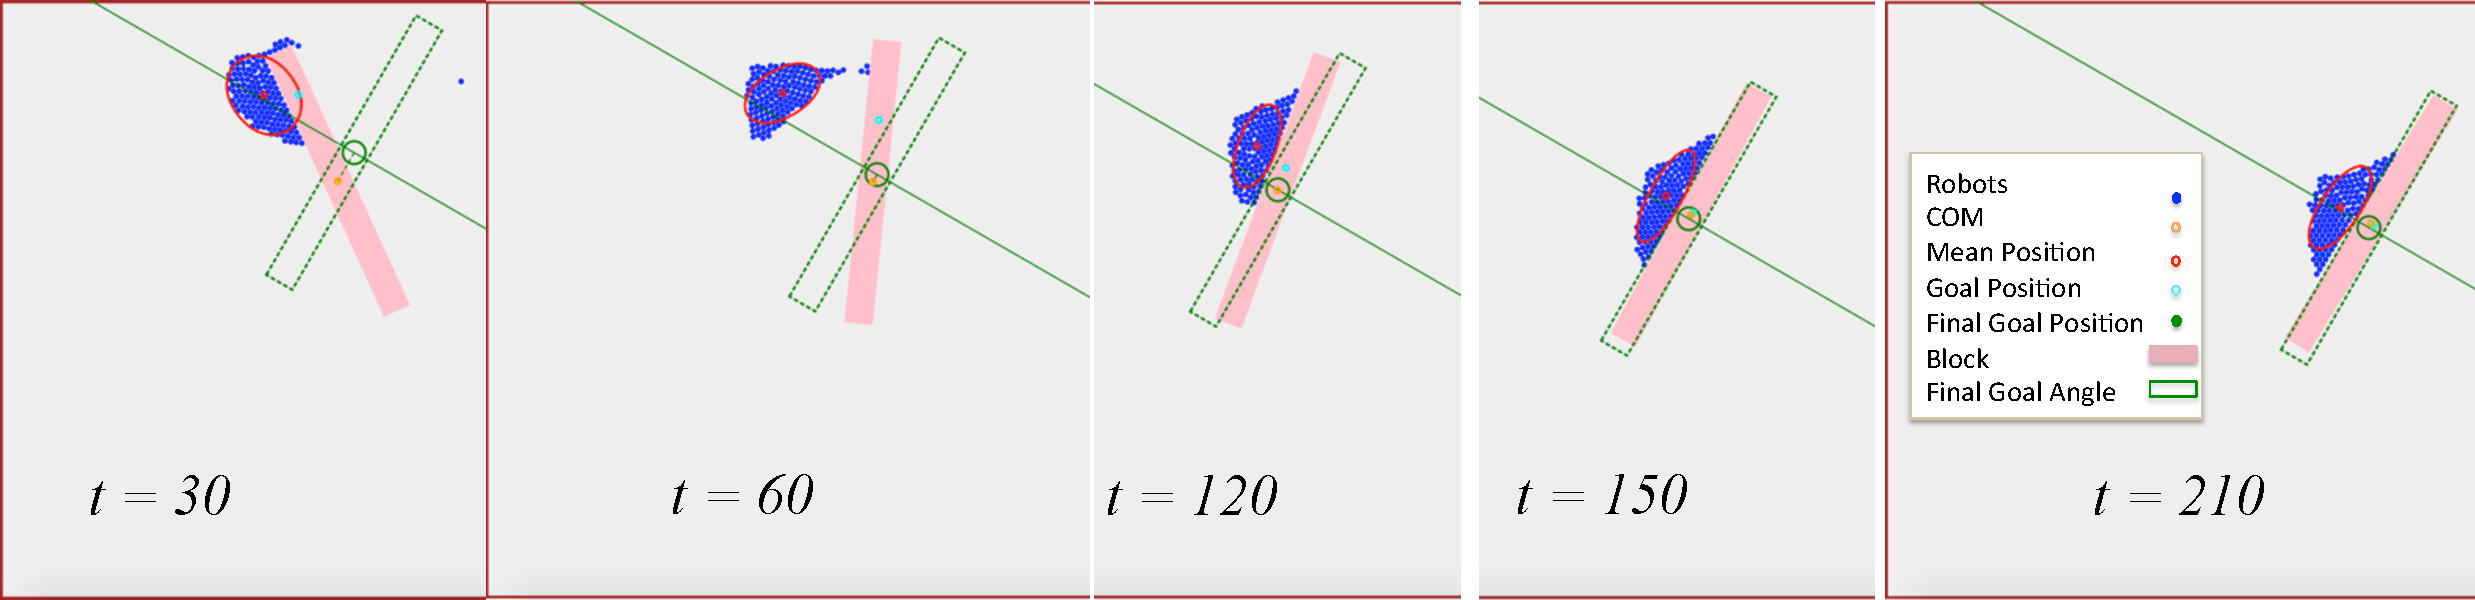
\includegraphics[width=2\columnwidth]{Linear.pdf}
\vspace{0em}
\caption{\label{fig:LinearScreenShots}
Screenshots from simulation of line following with perpendicular orientation.
 The object's COM is pushed to the line, while its orientation is regulated to be perpendicular to the line.
}
\end{figure*}
%TODO:  control law regulating distance from the straight line trajectory AND object orientation

%Perhaps: assume without loss of generality that the desired trajectory is the line $y = goal_y$

%\begin{align} \label{eq:StraightTrajectoryAndOrientation}
%goal_x &= O_x \nonumber \\
%goal_y &= O_y + K_\tau \Delta\theta  + K_p (O_y -  goal_y)
%\end{align}


%Shiva, you can do better than this, and write an equation to make the swarm follow an arbitrary line




\paragraph{Object pose control}
The section presents two algorithms designed to control the \emph{pose}, the position and orientation, of an object.  
Each works by first controlling the orientation and then regulating that orientation while translating the object. 

A na\"{i}ve approach might use pure translation moves by  pushing  the object with a contact point in line with the object's COM and the goal.
In practice the na\"{i}ve approach fails because the swarm has multiple points of contact. These contacts slide along the object, and the swarm flows around the object, usually splitting into multiple components as shown in Fig. \ref{fig:perpendicular}.
Instead, by applying force perpendicular to the object's long axis, splitting of the swarm is reduced. 

\begin{figure}
\begin{center}
	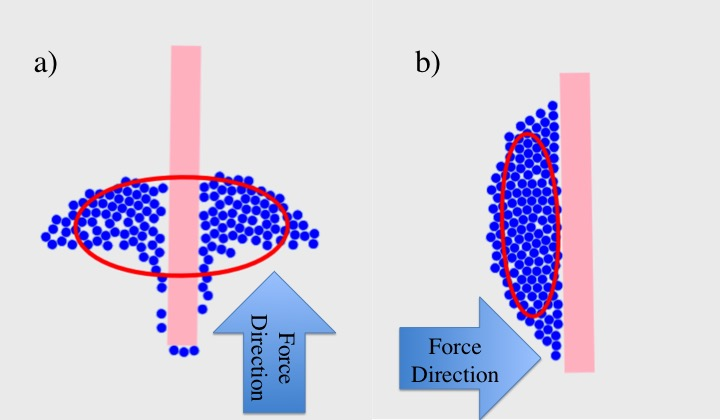
\includegraphics[width=\columnwidth]{perpendicular.jpg}
\end{center}
\vspace{-1em}
\caption{\label{fig:perpendicular} 
a.) Pushing an object perpendicular to its minor axis. The swarm spreads around the object. b.)  Applying force perpendicular to the object's long axis reduces the probability of splitting the swarm.
}
\vspace{-1em}
\end{figure}

The na\"{i}ve approach is represented in Alg. \ref{alg:naivePoseControlApproach}. It defines  the coordinate frame such that $[goal_x, goal_y, goal_{\theta}] = [0,0,0]$.
Then it cycles between regulating the angular error below some threshold $T_{\theta}$,
pushing the object along the major axis until position error perpendicular to the major axis is less than $T_x$, then pushing perpendicular to the minor axis until error perpendicular to the minor axis is less than $T_y$. 
This na\"{i}ve approach works poorly on objects with large aspect ratios because the swarm flows past the object, as shown in Fig.~\ref{fig:perpendicular}. 
Instead Alg. \ref{alg:PoseControl} seeks to always push the object perpendicular to the major axis, preventing the swarm from flowing around. 


\begin{algorithm}
\caption{PerpendicularPushesPoseControl}\label{alg:naivePoseControlApproach}
\begin{algorithmic}[1]
\Require $goal_x, goal_y, goal_{\theta},O_x, O_y, O_{\theta}$.
\State Define coordinate frame such that $[goal_x, goal_y, goal_{\theta}]^\top = [0,0,0]^\top$
\While {$\lvert O_x \rvert >T_x \vee \lvert O_y \rvert >T_y \vee \lvert O_{\theta} \rvert >T_{\theta}$}
	\While {$\lvert O_{\theta} \rvert >T_{\theta}$}
		\State Orientation control \S\ref{sec:simulation}.a
	\EndWhile
	\While {$\lvert O_x \rvert >T_{x}$}
		\State Straight translation \S\ref{sec:simulation}.c along line $y = 0$
	\EndWhile
	\While {$\lvert O_y \rvert >T_{y}$}
		\State Straight translation \S\ref{sec:simulation}.c along line $x = 0$
	\EndWhile
\EndWhile
\end{algorithmic}
\end{algorithm}



\begin{algorithm}
\caption{PoseControl}\label{alg:PoseControl}
\begin{algorithmic}[1]
\Require $goal_x, goal_y, goal_{\theta},O_x, O_y, O_{\theta}, C<1$.
\State $a = \cos(goal_{\theta})$ \Comment{Line Equation}
\State $b = \sin(goal_{\theta})$
\State $c = -a \cdot goal_x - b \cdot goal_y$

\Repeat 
\State $P_x = \frac{b(bO_x-aO_y)-a\cdot c}{a^2 + b^2}$  \Comment{Nearest point on line}
\State $P_y = \frac{a(-bO_x+aO_y)-b\cdot c}{a^2 + b^2}$
\State $\theta_t = goal_{\theta}+\pi/2$
\State $a_t = \cos(\theta_t )$ \Comment{Line Equation}
\State $b_t = \sin(\theta_t )$
\State $c_t = -a_t \cdot P_x - b_t \cdot P_y$
\State Line following with perpendicular orientation on line $(a_t,b_t,c_t)$  \S\ref{sec:simulation}.d
\State $d = \sqrt{(P_x-O_x)^2 + (P_y-O_y)^2}$
\Until {$d < C $} \Comment{Reaching near the line}
\State Line following with perpendicular orientation on line $(a,b,c)$ \S\ref{sec:simulation}.d
\end{algorithmic}
\end{algorithm}


Given a goal pose for the object, the algorithm constructs the line perpendicular to the long axis that intersects the goal pose. Alg.~\ref{alg:PoseControl} first moves the object to this line using the control law from \S\ref{sec:simulation}.d, then pushes the object to the goal pose using \S\ref{sec:simulation}.d.
%The swarm pushes the object to an intermediate location, from where a ``Line following with perpendicular orientation" move can deliver the object to the goal pose. 
A hysteresis-based variance control is used.  Whenever the swarm variance is bigger than a maximum variance threshold, the swarm is steered to  the corner to regather itself. 
This causes delays, but it usually prevents robots from flowing around the object. However, there is still some probability that a part of the swarm appears in front of the object, as shown in Fig. \ref{fig:PosControlFig} where at $t\approx170$ the orientation of the object is affected when the swarm is trying to regather because a group of the robots were in front of the object. Fig. \ref{fig:PosScreenShot} shows screenshots of the simulation. Simulation code that runs natively in any modern web browser is available at \cite{Shahrokhi16pose}.

\begin{figure}
\begin{center}
	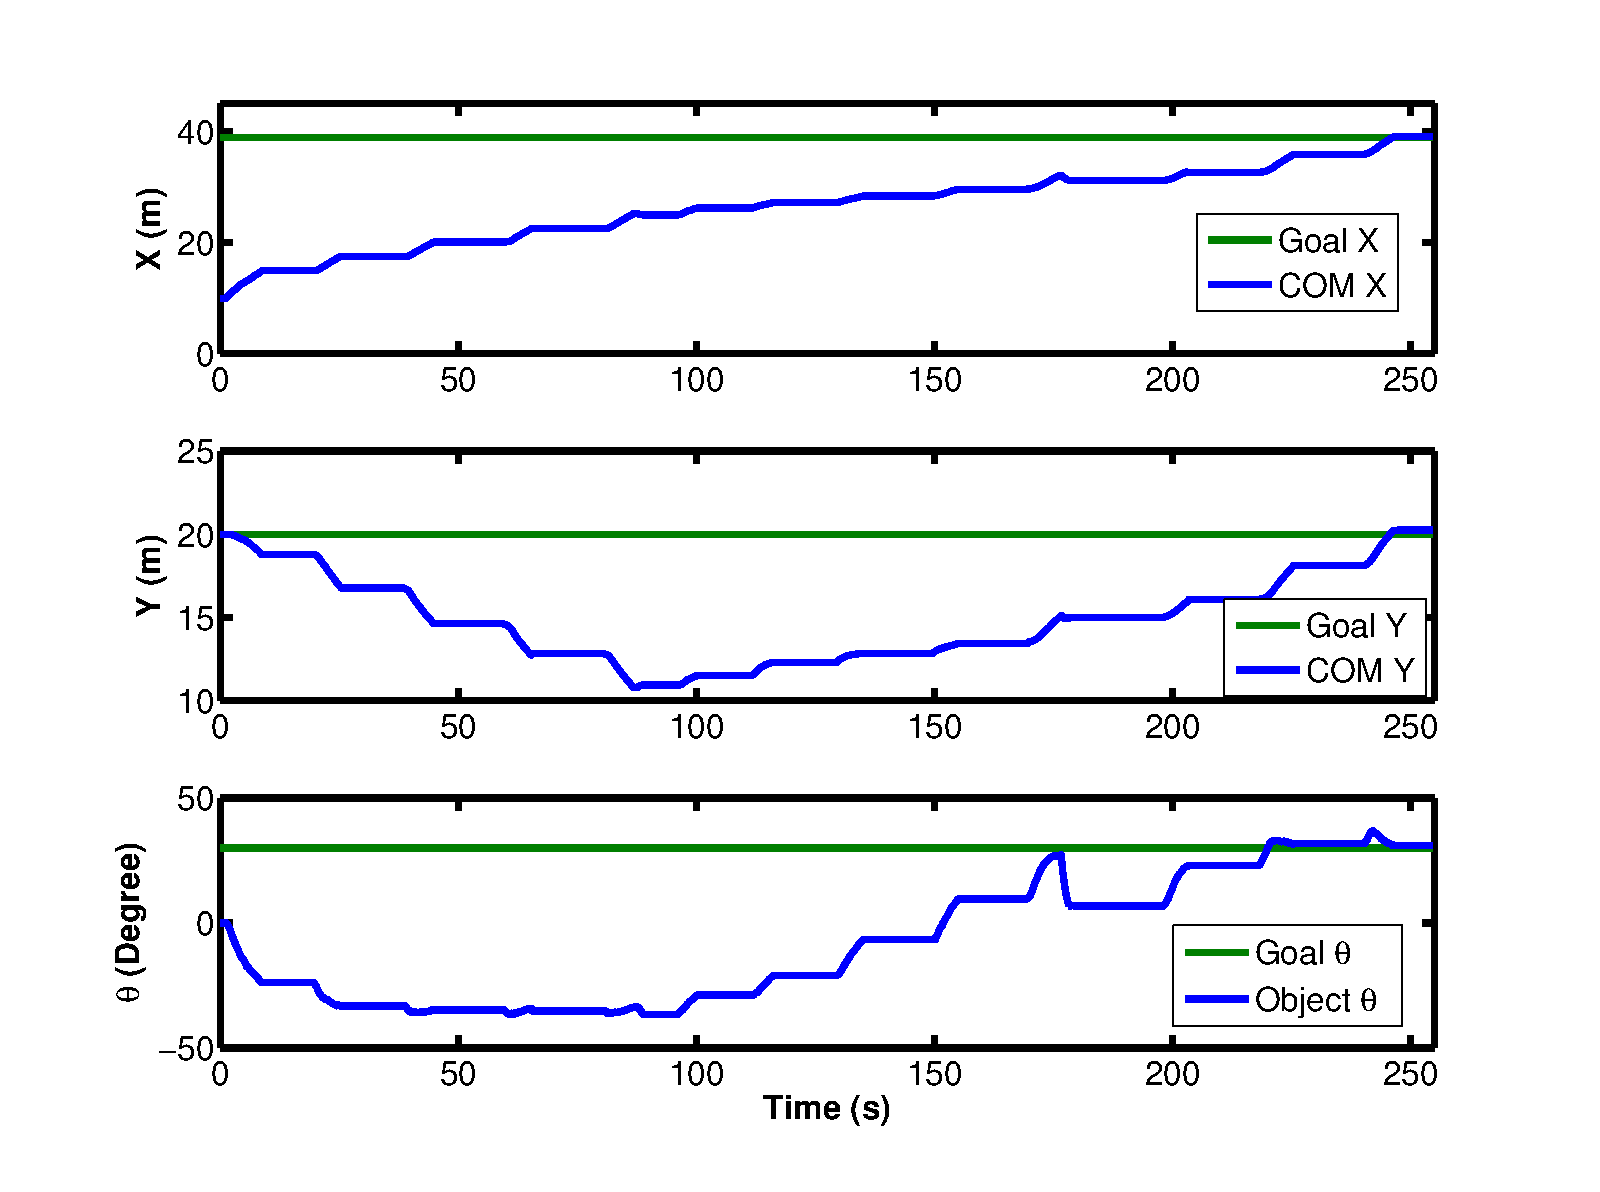
\includegraphics[width=1.07\columnwidth]{PosControl.eps}
\end{center}
\vspace{-2em}
\caption{\label{fig:PosControlFig} 
Pose control using Alg. \ref{alg:PoseControl}.  The objects is delivered to a goal position and orientation. The parts that the position including orientation is not changing, the swarm is in variance control mode to avoid splitting as much as it is possible. 
}
\vspace{-1em}
\end{figure}


\begin{figure*}
\centering

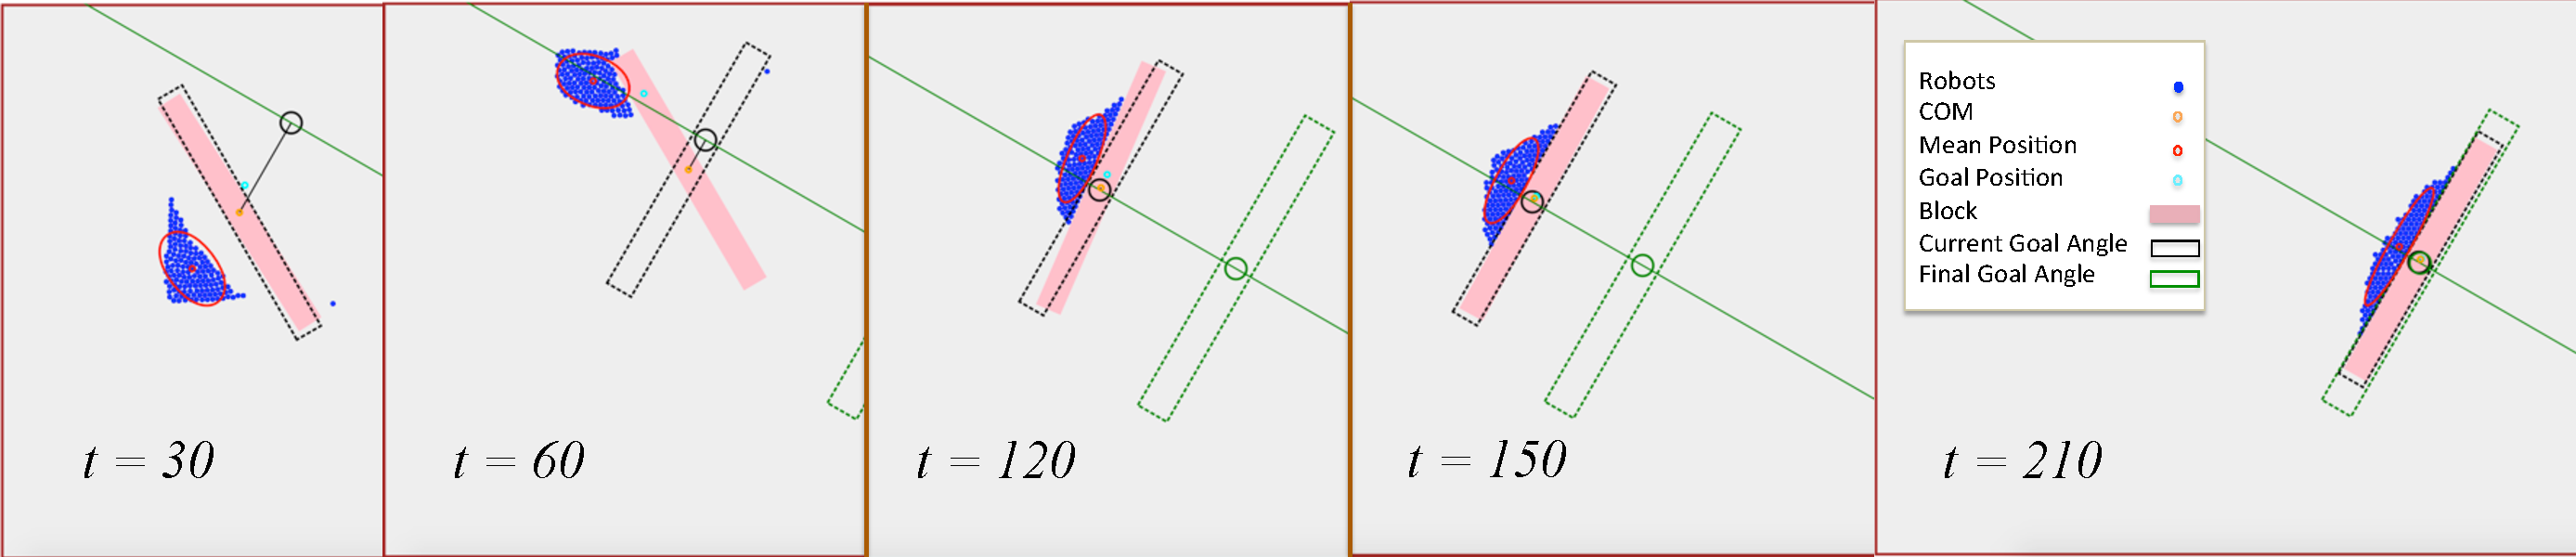
\includegraphics[width=2\columnwidth]{PoseControl.pdf}
\vspace{0em}
\caption{\label{fig:PosScreenShot}
Different stages for position control of a block while controlling its orientation. The first task (0--90 s) is to push the object COM to a line perpendicular to the goal. The second task (90--210 s) is to push the object along this perpendicular line while regulating the orientation.
}
\end{figure*}


